\documentclass{article}
\usepackage[margin=1in]{geometry}
\usepackage{amsmath}
\usepackage{amssymb}
\usepackage{graphicx}

\title{Tiny Shakespeare Transformer Report}
\author{Aarush Ram Anandh}
\date{\today}

\begin{document}
\maketitle

\section*{Implementation Architecture}
The notebook implements a minimal Transformer language model using plain PyTorch tensors and functions rather than a full \texttt{nn.Module} class. Parameters are stored in nested Python dictionaries. The model maps a sequence of character indices to logits over the vocabulary. The flow is:
\begin{enumerate}
	\item Read text, build a character vocabulary, and encode the text into integer tokens.
	\item Embed tokens and positions, sum them, then apply a stack of Transformer blocks.
	\item Apply a final layer norm and a linear output projection to produce logits.
	\item Train with cross entropy loss and Adam optimizer.
	\item Run inference by autoregressive sampling from the output distribution.
\end{enumerate}

\section*{Causal Mask Construction}
The mask prevents attention to future positions. The code creates an upper-triangular matrix and fills it with $-\infty$ above the diagonal:
\[
M = \text{triu}(\mathbf{1}_{T \times T}, 1), \quad M_{ij} = \begin{cases}-\infty & i < j \\ 0 & \text{otherwise}\end{cases}
\]
This is added to the attention scores before softmax so future tokens get zero probability.

\section*{How $W_q$, $W_k$, and $W_v$ Are Built}
For each attention head $h$, the notebook initializes learnable matrices with scaled Gaussian noise:
\[
W_q^{(h)}, W_k^{(h)}, W_v^{(h)} \in \mathbb{R}^{d_h \times d_h}, \quad W \sim \mathcal{N}(0, 1) / \sqrt{d}
\]
where $d_h$ is the head dimension and $d$ is the embedding size. The output projection $W_o \in \mathbb{R}^{d \times d}$ is initialized similarly.

\section*{Transformer Arrangement}
Each block contains multi-head attention and a feedforward network, each wrapped with residual connections and layer normalization:
\[
\text{Block}(x) = \text{LN}_2\big(\text{LN}_1(x + \text{MHA}(x)) + \text{FFN}(\text{LN}_1(x + \text{MHA}(x)))\big)
\]
The model stacks \texttt{num\_layers} of these blocks, then applies a final layer norm and a linear output projection.

\section*{Function Definitions (Mathematical Form)}
Below, each function is described as a mathematical mapping with its inputs and outputs.

\subsection*{\texttt{load\_text}}
\[
\mathrm{load\_text}(p) = (x, \mathrm{stoi}, \mathrm{itos}, V)
\]
Read text $s$ from path $p$, build vocabulary $C$, and map each character to an index:
\[
x_i = \mathrm{stoi}(s_i), \quad V = |C|
\]

\subsection*{\texttt{get\_batch}}
Given data $x \in \mathbb{Z}^N$, batch size $B$, and block size $T$:
\[
\mathrm{get\_batch}(x, B, T) = (X, Y)
\]
where
\[
X_{b,t} = x_{i_b + t}, \quad Y_{b,t} = x_{i_b + t + 1}
\]
and $i_b$ are random start indices.

\subsection*{\texttt{create\_causal\_mask}}
\[
\mathrm{create\_causal\_mask}(T) = M \in \mathbb{R}^{T \times T}
\]
with $M_{ij} = -\infty$ for $i < j$ and $0$ otherwise.

\subsection*{\texttt{self\_attention}}
For input $x \in \mathbb{R}^{B \times T \times d_h}$ and weights $W_q, W_k, W_v$:
\[
Q = x W_q, \quad K = x W_k, \quad V = x W_v
\]
\[
S = \frac{QK^\top}{\sqrt{d_h}} + M, \quad A = \mathrm{softmax}(S)
\]
\[
\mathrm{self\_attention}(x) = AV
\]

\subsection*{\texttt{multi\_head\_attention}}
Split $x$ into $H$ heads and apply \texttt{self\_attention} per head:
\[
\mathrm{MHA}(x) = \big[\mathrm{SA}_1(x_1) \; || \; \dots \; || \; \mathrm{SA}_H(x_H)\big] W_o
\]
where $||$ denotes concatenation.

\subsection*{\texttt{feedforward}}
\[
\mathrm{FFN}(x) = \mathrm{ReLU}(x W_1) W_2
\]

\subsection*{\texttt{transformer\_block}}
\[
u = x + \mathrm{MHA}(x), \quad v = \mathrm{LN}_1(u)
\]
\[
z = v + \mathrm{FFN}(v), \quad \mathrm{Block}(x) = \mathrm{LN}_2(z)
\]

\subsection*{\texttt{forward}}
For token indices $x \in \mathbb{Z}^{B \times T}$:
\[
e = E_{tok}(x) + E_{pos}(0{:}T-1)
\]
\[
h = \mathrm{Block}_L(\dots \mathrm{Block}_1(e)\dots)
\]
\[
\mathrm{forward}(x) = h W_{out}
\]

\subsection*{\texttt{compute\_loss}}
\[
\mathrm{compute\_loss}(\ell, y) = \mathrm{CE}(\ell, y)
\]
where $\ell$ are logits and $y$ are target indices.

\subsection*{\texttt{train}}
Given parameters $\theta$, the update per step is:
\[
(X, Y) = \mathrm{get\_batch}(x, B, T)
\]
\[
\ell = \mathrm{forward}(X), \quad L = \mathrm{CE}(\ell, Y)
\]
\[
\theta \leftarrow \mathrm{Adam}(\theta, \nabla_\theta L)
\]

\subsection*{\texttt{generate}}
For start tokens $s$ and steps $N$:
\[
\text{for } t=1..N: \quad \ell = \mathrm{forward}(x_{\text{last }T}),\; p = \mathrm{softmax}(\ell_{-1}),\; x \leftarrow [x, \mathrm{sample}(p)]
\]

\section*{Function Call Flow}
\begin{itemize}
	\item Training cell: \texttt{load\_text} $\rightarrow$ \texttt{init\_params} $\rightarrow$ \texttt{train}.
	\item Inside \texttt{train}: \texttt{get\_batch} $\rightarrow$ \texttt{forward} $\rightarrow$ \texttt{compute\_loss} $\rightarrow$ optimizer step.
	\item Inference cell: \texttt{load\_text} $\rightarrow$ load \texttt{params} $\rightarrow$ \texttt{generate}.
	\item Extended training cell: load \texttt{params} $\rightarrow$ \texttt{train} for more steps.
\end{itemize}

\section*{Training Procedure and Torch Operations}
Training uses only core PyTorch operations: tensor indexing, \texttt{torch.randint}, \texttt{torch.stack}, \texttt{torch.triu}, \texttt{masked\_fill}, \texttt{softmax}, \texttt{cross\_entropy}, and \texttt{torch.optim.Adam}. Gradients are computed with \texttt{loss.backward()} and parameters are updated with \texttt{optimizer.step()}.

\section*{Input Text Embedding}
Embedding does occur. Tokens are mapped to indices and passed through \texttt{nn.Embedding} to produce vectors in $\mathbb{R}^d$. A positional embedding of size \texttt{block\_size} is added:
\[
E(x) = E_{tok}(x) + E_{pos}(0{:}T-1)
\]
This sum is the Transformer input.

\section*{Results}
\subsection*{Loss Curve}
\begin{figure}[h]
	\centering
	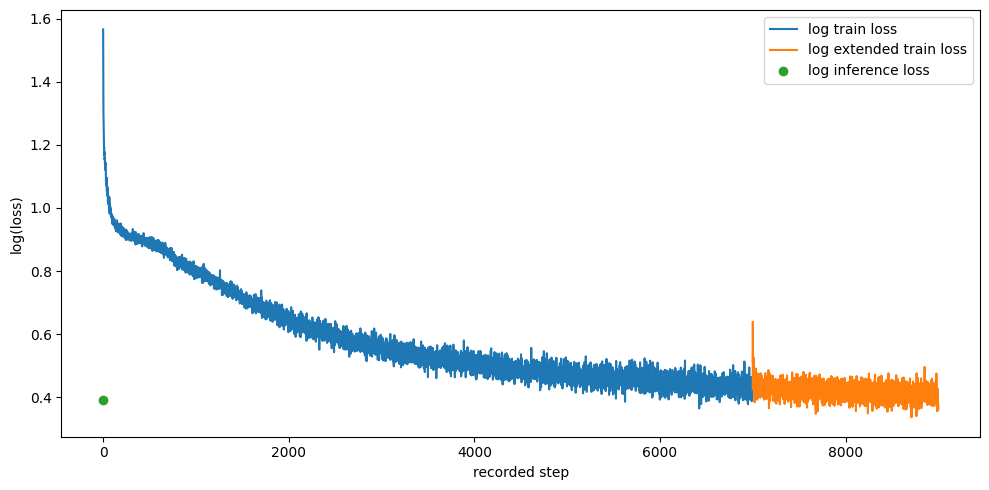
\includegraphics[width=\linewidth]{loss_curve.png}
	\caption{Training and extended training loss over recorded steps.}
\end{figure}
The loss decreases steadily from the initial high value and flattens as training progresses, indicating improved next-character prediction. The extended training continues from the end of the main curve and shows smaller incremental gains.

\subsection*{Inference Samples}
\textbf{Sample 1 (standard inference cell)}
\begin{verbatim}
HASLENCE:
Is I with that him art.

BIONDELLO:
Can the therefore; but my hearty him, high nobless
Talk the satish his bend; in jurtiful wom
To not; for have you to thy womand's diam;
Assarrione this donter, at now hereth,
Lifttor: I'll are galeth art poor with our thy toook.
That shall ever, sad do in
\end{verbatim}

\textbf{Sample 2 (custom prompt cell, with inference loss $\approx 1.48$)}
\begin{verbatim}
hi wowan king'd.
Methink; by be younger a dayswors cunking,
My fathen I'll statingly.

Nill ELifne:
Having to please take the forgetn, blish the gods
The veryoners outacher'd countaly justing time,
And coursent silf a chasqued homicted
In much a dame: I concin of your know
her rearn than breast your city, m
\end{verbatim}

\subsection*{Inference Quality}
The model shows recognizable Shakespeare-like structure (character names, line breaks, and archaic tone) but still produces many non-words and malformed phrases. This is typical for a small model trained at character level. Longer training and larger model capacity would likely improve grammatical coherence and reduce gibberish tokens.

\end{document}
